\documentclass[border=5pt,tikz]{standalone}
\usepackage{tikz}
\usepackage{xcolor}
\usepackage{amsmath,amssymb}

\definecolor{darknavy}{HTML}{122128}
\definecolor{forgisorange}{HTML}{FF5A00}
\definecolor{panelbg}{HTML}{F0F4F8}
\definecolor{figsteel}{HTML}{878F92}

\usetikzlibrary{arrows.meta, positioning, calc}

\begin{document}
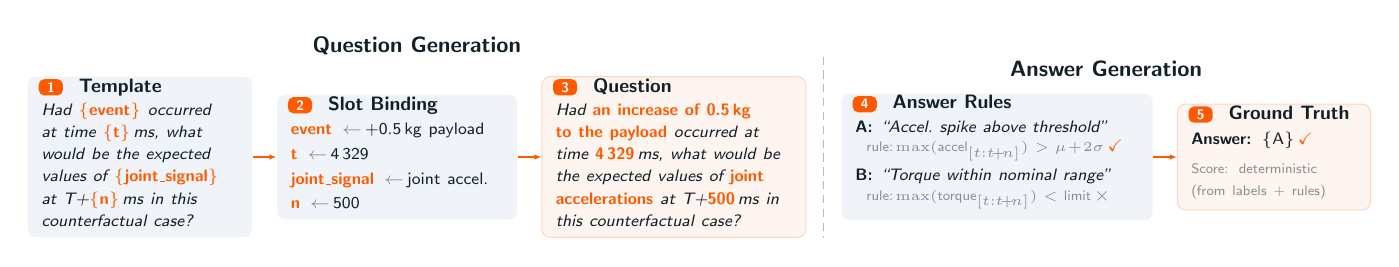
\begin{tikzpicture}[
    font=\sffamily\scriptsize\color{darknavy},
    arr/.style={
        -{Latex[length=2.5pt, width=2pt]},
        forgisorange, line width=0.7pt,
    },
    stdpanel/.style={
        rectangle, rounded corners=3pt, fill=panelbg,
        inner xsep=5pt, inner ysep=4pt, align=left,
    },
    outpanel/.style={
        rectangle, rounded corners=3pt,
        fill=forgisorange!6, draw=forgisorange!25, line width=0.4pt,
        inner xsep=5pt, inner ysep=4pt, align=left,
    },
    badge/.style={
        fill=forgisorange, rounded corners=2pt,
        inner xsep=3pt, inner ysep=1.2pt,
        font=\sffamily\bfseries\tiny, text=white,
        anchor=west,
    },
    boxtitle/.style={
        font=\sffamily\bfseries\scriptsize, text=darknavy,
        anchor=base west,
    },
]

% -- Box 1: Template --
\node[stdpanel, text width=2.5cm, anchor=north west] (b1) at (0,0) {%
    {\rule{0pt}{8pt}}\\[-6pt]
    {\fontsize{6}{7.8}\selectfont\itshape
        Had {\bfseries\color{forgisorange}\{event\}} occurred at time
        {\bfseries\color{forgisorange}\{t\}}\,ms, what would be the
        expected values of {\bfseries\color{forgisorange}\{joint\_signal\}}
        at T+{\bfseries\color{forgisorange}\{n\}}\,ms in this counterfactual case?}%
};
\node[badge] (bg1) at ([xshift=4pt, yshift=-4pt]b1.north west) {\textsc{1}};
\node[boxtitle] at ([xshift=2pt]bg1.base east) {Template};

% -- Box 2: Slot Binding --
\node[stdpanel, text width=2.7cm, right=0.3cm of b1] (b2) {%
    {\rule{0pt}{8pt}}\\[-6pt]
    {\fontsize{6}{8.5}\selectfont
        {\bfseries\color{forgisorange}event}
            {\color{figsteel}\,$\leftarrow$\,}+0.5\,kg payload\\[0.5pt]
        {\bfseries\color{forgisorange}t}
            {\color{figsteel}\,$\leftarrow$\,}4\,329\\[0.5pt]
        {\bfseries\color{forgisorange}joint\_signal}
            {\color{figsteel}\,$\leftarrow$\,}joint accel.\\[0.5pt]
        {\bfseries\color{forgisorange}n}
            {\color{figsteel}\,$\leftarrow$\,}500}%
};
\node[badge] (bg2) at ([xshift=4pt, yshift=-4pt]b2.north west) {\textsc{2}};
\node[boxtitle] at ([xshift=2pt]bg2.base east) {Slot Binding};

% -- Box 3: Instantiated Question --
\node[outpanel, text width=3.0cm, right=0.3cm of b2] (b3) {%
    {\rule{0pt}{8pt}}\\[-6pt]
    {\fontsize{6}{7.8}\selectfont\itshape
        Had {\bfseries\color{forgisorange}an increase of 0.5\,kg to the payload}
        occurred at time {\bfseries\color{forgisorange}4\,329}\,ms, what would be
        the expected values of {\bfseries\color{forgisorange}joint accelerations}
        at T+{\bfseries\color{forgisorange}500}\,ms in this counterfactual case?}%
};
\node[badge] (bg3) at ([xshift=4pt, yshift=-4pt]b3.north west) {\textsc{3}};
\node[boxtitle] at ([xshift=2pt]bg3.base east) {Question};

% -- Arrows left half --
\draw[arr] (b1.east) -- (b2.west);
\draw[arr] (b2.east) -- (b3.west);

% ============ DIVIDER ============
\coordinate (divtop) at ($(b3.north east) + (0.22, 0.25)$);
\coordinate (divbot) at ($(b3.south east) + (0.22, 0)$);
\draw[figsteel!60, densely dashed, line width=0.5pt] (divtop) -- (divbot);

% -- Box 4: Answer Rule Pool --
\node[stdpanel, text width=3.6cm, right=0.44cm of b3] (b4) {%
    {\rule{0pt}{8pt}}\\[-6pt]
    {\fontsize{6}{8}\selectfont
        \textbf{A:} \textit{``Accel.\ spike above threshold''}\\[-1pt]
        \hspace*{4pt}{\fontsize{5}{7}\selectfont\color{figsteel}
            rule:\,$\max(\text{accel}_{[t:t\!+\!n]}) > \mu\!+\!2\sigma$}\,{\color{forgisorange}\checkmark}\\[2.5pt]
        \textbf{B:} \textit{``Torque within nominal range''}\\[-1pt]
        \hspace*{4pt}{\fontsize{5}{7}\selectfont\color{figsteel}
            rule:\,$\max(\text{torque}_{[t:t\!+\!n]}) < \text{limit}$}\,{\color{figsteel}$\times$}}%
};
\node[badge] (bg4) at ([xshift=4pt, yshift=-4pt]b4.north west) {\textsc{4}};
\node[boxtitle] at ([xshift=2pt]bg4.base east) {Answer Rules};

% -- Box 5: Ground-Truth Answer --
\node[outpanel, text width=2.1cm, right=0.3cm of b4] (b5) {%
    {\rule{0pt}{8pt}}\\[-6pt]
    {\fontsize{6}{8.5}\selectfont
        \textbf{Answer:} \{A\}\,{\color{forgisorange}\checkmark}\\[3pt]
        {\fontsize{5.5}{7.5}\selectfont\color{figsteel}
            Score: deterministic\\(from labels + rules)}}%
};
\node[badge] (bg5) at ([xshift=4pt, yshift=-4pt]b5.north west) {\textsc{5}};
\node[boxtitle] at ([xshift=2pt]bg5.base east) {Ground Truth};

% -- Arrow right half --
\draw[arr] (b4.east) -- (b5.west);

% ============ SECTION TITLES ============
\node[font=\sffamily\bfseries\footnotesize, text=darknavy, anchor=south]
    at ($(b1.north west)!0.5!(b3.north east) + (0, 0.15)$)
    {Question Generation};

\node[font=\sffamily\bfseries\footnotesize, text=darknavy, anchor=south]
    at ($(b4.north west)!0.5!(b5.north east) + (0, 0.15)$)
    {Answer Generation};

\end{tikzpicture}
\end{document}
